\chapter{How To Qualify A Good Company To Invest In}

The question is simple, but it is not small: what do we look for in a company that we would really want to invest in? The answer in this interview does not begin with a valuation formula or a heroic story about founders. It begins with mandate, stage, and scale. We first locate the investor, then we locate the kind of company, and only then do we ask what makes that company worth attention.

\section{The Question Of Qualification}

The opening question asks for a rule of judgment. In a mature business, we might begin with profit, cash flow, leverage, or market share. Here the setting is earlier. The speaker describes a group with capital to deploy and a venture orientation, so the evidence is necessarily incomplete. The investment decision has to be made before the company has become fully legible.

We can write the problem schematically as follows. For a candidate company \(X\), the investor is not asking for a single number. The investor is asking whether several early signals line up:
\begin{equation}
X \longmapsto
\left(
\hbox{idea},
\hbox{team},
\hbox{market},
\hbox{stage},
\hbox{support needed}
\right).
\end{equation}
This notation is only a compact way to preserve the interview's sequence. The transcript gives us no formal scoring model. The useful discipline is that the question is not ``Is this company exciting?'' but ``Is this company exciting in the right stage, at the right size, with the right kind of help available?''

\subsection{Question \& Answer}

\paragraph{Question.}
What are some things that we look for in a company that we really want to invest in?

\paragraph{Answer.}
We begin with the investor's own frame. The group has about \( \$50\,\text{M} \) to invest, is considered venture, and works in very early rounds. Within that frame, the speaker names three screens: really interesting ideas, thoughtful management teams, and large target markets. Then the answer becomes numerical: typical investments are somewhere between about half a million dollars and perhaps two or three million dollars, and the companies are probably generating less than \( \$2\,\text{M} \) in revenue. Finally, the answer becomes operational: after investing, the group helps the company get organized, hire strong talent, and stay focused.

\section{Mandate Before Criteria}

The first important move is that the speaker does not begin with taste. He begins with the capital base. The group has about
\begin{equation}
F \approx \$50\,\text{M}
\end{equation}
to invest. That number is not merely decorative. A fund or investment group of that scale cannot behave like a public-market investor buying tiny positions in mature companies, and it also cannot behave like a massive late-stage fund that requires very large checks to matter.

The mandate tells us what sort of evidence will count. In a very early company, the clean financial ratios may be thin or absent. A young company may have revenue, but not enough history to let the numbers settle the case by themselves. So the investor's reasoning has to combine rough quantitative boundaries with qualitative judgment.

The speaker then names the category: venture, very early rounds. This narrows the terrain. We are not yet in the world where the only question is whether this year's earnings justify this year's price. We are in the world where an investor asks whether the early shape of the company could grow into something much larger.

\section{The Early-Stage Screen}

Once the stage is fixed, the screen comes in three parts:
\begin{equation}
\mathcal{S}(X)
=
\left\{
\hbox{interesting idea},
\hbox{thoughtful management team},
\hbox{large target market}
\right\}.
\end{equation}
Again, \(\mathcal{S}\) is our notation, not the speaker's. It is useful because it keeps the three claims together without pretending that they are a mechanical formula.

The first term is the idea. At this stage, the idea matters because the company may not yet have enough scale for the accounting record to carry the whole argument. But an idea by itself is not enough. The second term is the management team. The speaker says ``thoughtful'' management teams, which is a different claim from merely energetic or charismatic teams. Thoughtfulness points toward judgment, prioritization, and the capacity to learn under pressure.

The third term is the target market. Venture investing needs room. A small idea can be a good business, but a venture investment normally needs a market large enough to absorb growth. In this sequence, market size is not an abstraction added later by a textbook writer. It is part of the initial answer: idea, team, market.

\section{The Size Of The Bet}

After the qualitative screen, the speaker turns to the size of the investment. Most investments are described as somewhere between half a million dollars and maybe two or three million dollars:
\begin{equation}
C \approx \$0.5\,\text{M}
\quad \hbox{to} \quad
\$2\text{M--}3\,\text{M}.
\end{equation}
The upper end should be read cautiously. The phrase ``maybe two or three million dollars'' is not a sharp mathematical boundary. It is a spoken range that tells us the order of magnitude of the commitment.

Still, the range has meaning. A check of \( \$0.5\,\text{M} \) to \( \$3\,\text{M} \) is large enough to influence a small company, but small enough to belong naturally to early-stage venture. The investment is not merely a passive purchase. It is capital placed into a company where the investor may also help shape focus, hiring, and organization.

A compact stage condition can be written as
\begin{equation}
\hbox{early-stage fit}
\quad \Longleftrightarrow \quad
\left(
C \hbox{ is on the order of } \$0.5\text{M--}3\text{M}
\right)
\hbox{ and }
\left(
R \lesssim \$2\,\text{M}
\right),
\end{equation}
where \(R\) denotes company revenue. This is not a valuation theorem. It is a disciplined summary of the spoken boundaries.

\section{Revenue Stage And Operating Reality}

The companies are described as generating probably less than \( \$2\,\text{M} \) in revenue:
\begin{equation}
R \lesssim \$2\,\text{M}.
\end{equation}
The word ``probably'' matters. We should not convert this into a rigid cutoff. The important point is stage. These companies have enough reality to be companies, but not enough maturity to be left alone as finished machines.

This explains why the earlier criteria look the way they do. If \(R\) is still below about \( \$2\,\text{M} \), then the investor cannot reduce the company to a mature financial profile. The team has to matter. The market has to matter. The idea has to matter. And the investor has to ask what kind of help would make the company more coherent.

Here is a small example, using only the interview's ranges. Suppose a candidate company has revenue
\[
R_X = \$1.4\,\text{M}
\]
and is raising
\[
C_X = \$1.0\,\text{M}.
\]
Numerically, it sits inside the described region:
\begin{align}
R_X &= \$1.4\,\text{M} < \$2\,\text{M},\\
C_X &= \$1.0\,\text{M} \in [\$0.5\,\text{M},\, \$2\text{M--}3\,\text{M}].
\end{align}
That does not mean the company is investable. It only means the company is in the right neighborhood for this kind of investor. The remaining questions are the ones the speaker has already named: is the idea interesting, is the management team thoughtful, and is the target market large?

\section{From Selection To Support}

The answer does not stop at choosing companies. The speaker says that after making these investments, they focus the companies, get them organized, help them hire really good talent, and make sure they stay focused on the right things. We can summarize the support mechanism as
\begin{equation}
\mathcal{H}
=
\left\{
\hbox{organize},
\hbox{hire talent},
\hbox{focus}
\right\}.
\end{equation}
This is the second half of the investment logic. The investor is not only screening from the outside. The investor expects to affect the company's operating path.

The reason appears in the final movement of the transcript. A young entrepreneur or CEO has too many things coming at once and too few people to deal with them. The bottleneck is not only money. It is attention. A young company can fail because the idea is weak, but it can also fail because the important work is buried under a flood of urgent work.

The practical update rule is therefore simple:
\begin{equation}
\hbox{post-investment priority}
\quad \longrightarrow \quad
\hbox{increase focus, increase talent, reduce confusion}.
\end{equation}
That is not a mathematical law. It is the operating mechanism that connects the check to the company's next stage.

\begin{figure}
\centering
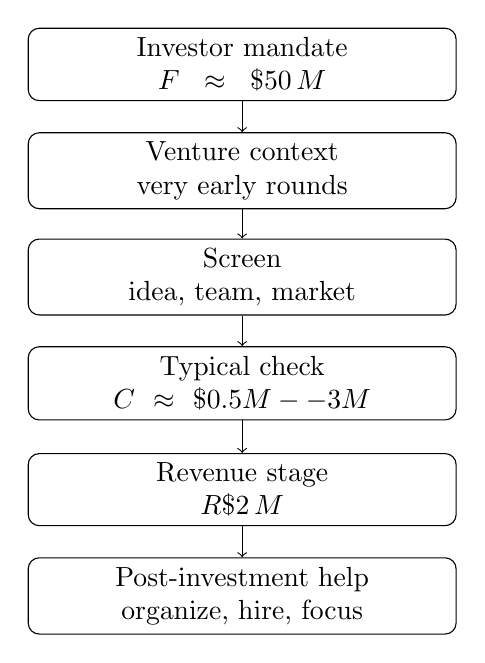
\begin{tikzpicture}[x=1cm,y=1cm]
\node[draw, rounded corners, align=center, text width=5.2cm] (a) at (0,0) {Investor mandate\\ \(F \approx \$50\,\text{M}\)};
\node[draw, rounded corners, align=center, text width=5.2cm] (b) at (0,-1.35) {Venture context\\ very early rounds};
\node[draw, rounded corners, align=center, text width=5.2cm] (c) at (0,-2.70) {Screen\\ idea, team, market};
\node[draw, rounded corners, align=center, text width=5.2cm] (d) at (0,-4.05) {Typical check\\ \(C \approx \$0.5\text{M--}3\text{M}\)};
\node[draw, rounded corners, align=center, text width=5.2cm] (e) at (0,-5.40) {Revenue stage\\ \(R \lesssim \$2\,\text{M}\)};
\node[draw, rounded corners, align=center, text width=5.2cm] (f) at (0,-6.75) {Post-investment help\\ organize, hire, focus};

\draw[->] (a) -- (b);
\draw[->] (b) -- (c);
\draw[->] (c) -- (d);
\draw[->] (d) -- (e);
\draw[->] (e) -- (f);
\end{tikzpicture}
\caption{A transcript-derived reconstruction of the investment sequence. No board diagram was preserved for this lecture; the figure organizes the spoken order for note-taking.}
\end{figure}

\section{Summary}

The interview gives us a compact model of early-stage investment judgment. First, locate the investor: about \( \$50\,\text{M} \) to invest, operating as venture capital in very early rounds. Then locate the company: an interesting idea, a thoughtful team, a large target market, a check size around \( \$0.5\,\text{M} \) to \( \$2\text{M--}3\,\text{M} \), and revenue probably below \( \$2\,\text{M} \).

The final lesson is that qualification and assistance belong together. The investor looks for a company that fits the stage and has the raw ingredients, but the work after investment is to help the young CEO organize the company, hire talent, and stay focused when too many demands arrive at once.